\begin{subfigure}[t]{\textwidth}
    \centering
    \begin{subfigure}[t]{\textwidth}
\centering
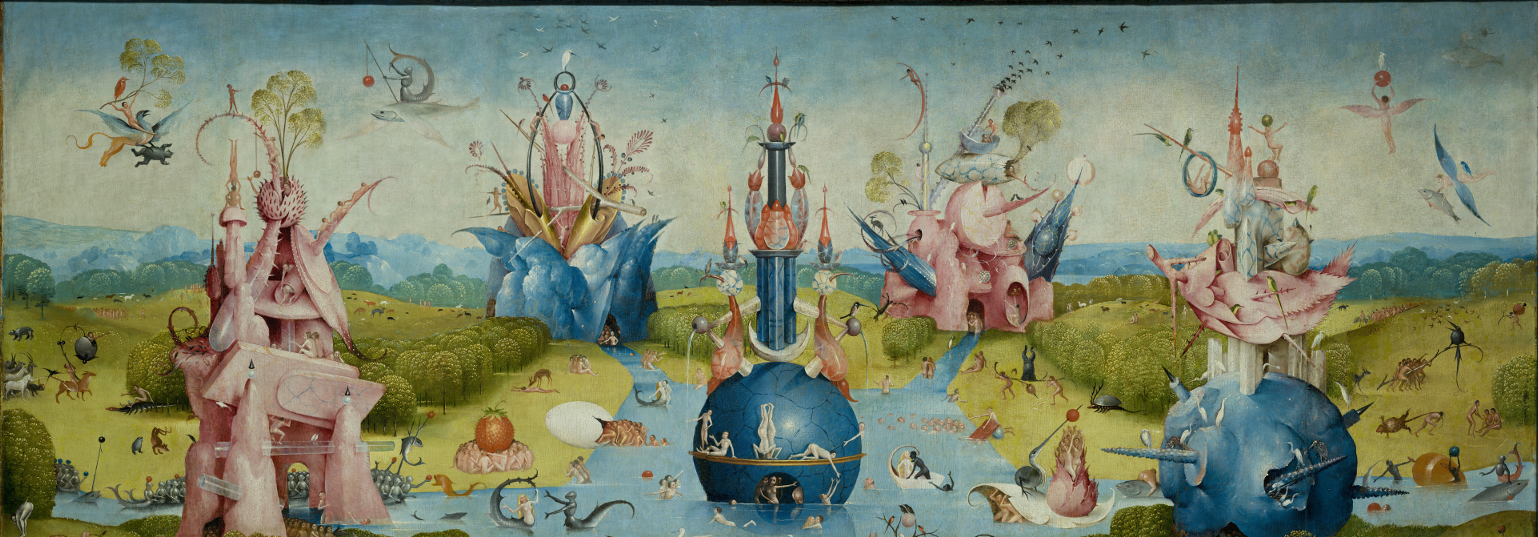
\includegraphics[width=\textwidth]{images/B1.png}
\label{fig.b1}
\caption{Les cinq structures font office d'instrument de musique spatialisé : chacun produira un son à une hauteur différente. Lorsque le premier est activé, des effets commencent à s'appliquer sur le son.}
    \end{subfigure}~\\   
    \begin{subfigure}[t]{\textwidth}
\centering
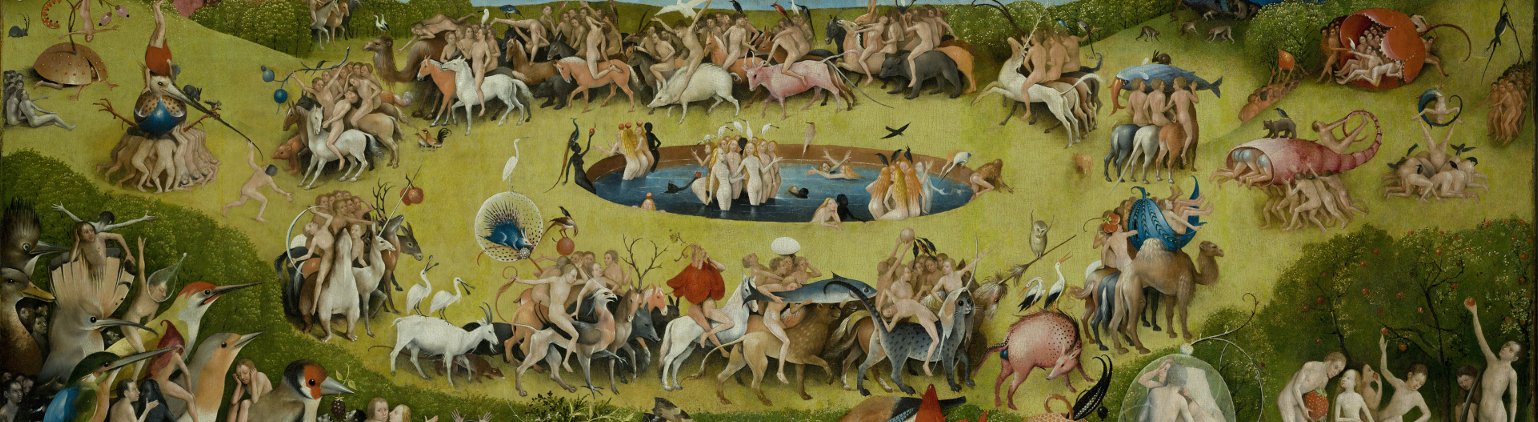
\includegraphics[width=\textwidth]{images/B2.png}
\caption{Il est possible d'explorer cette scène en naviguant dans son espace; le mouvement invite à l'utilisation de trajectoires spatialisées qui sont implémentées à l'aide d'automations tridimensionnelles dans i-score.}
\label{fig.b2}
    \end{subfigure}~\\  
    \begin{subfigure}[t]{\textwidth}
\centering
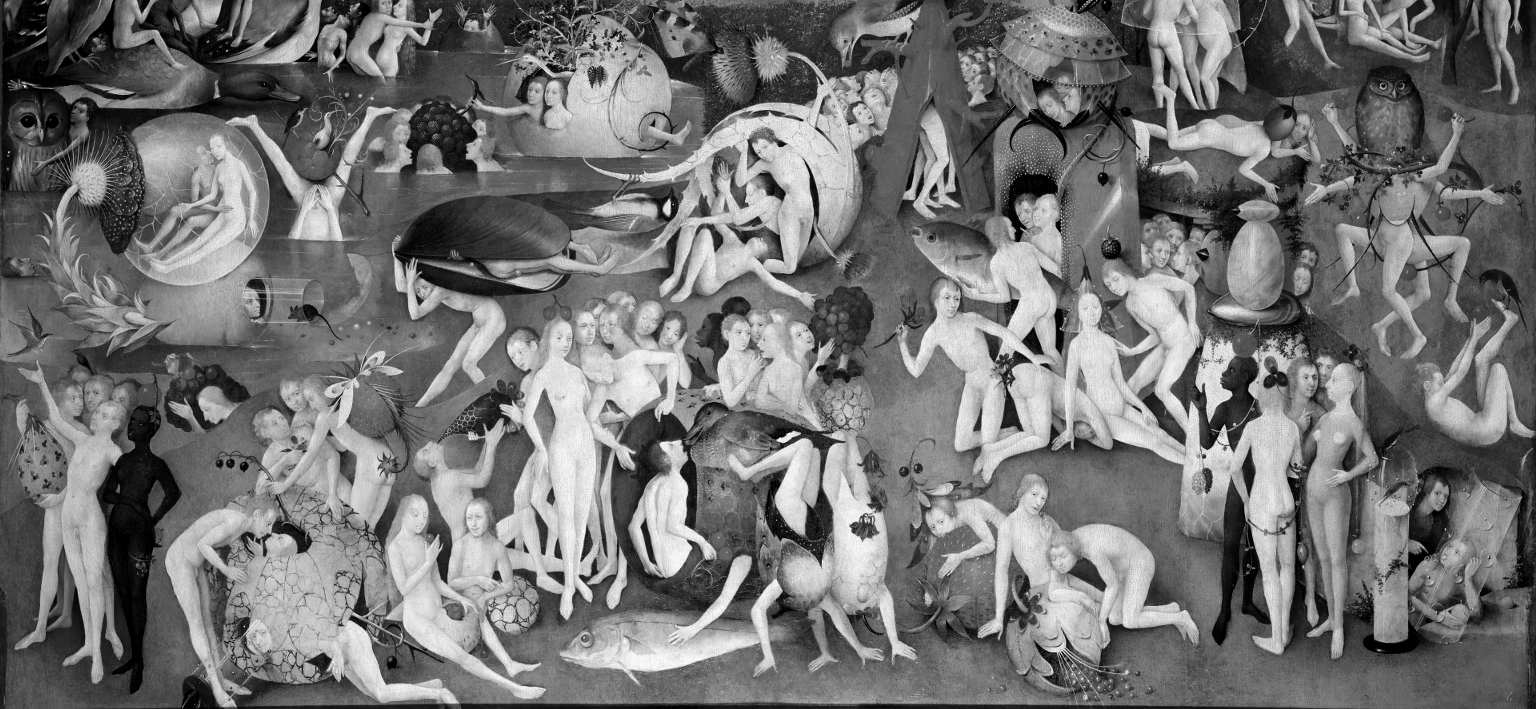
\includegraphics[width=\textwidth]{images/B3.png}
\caption{Dans cette partie, des acteurs se déplacent en permanence; interagir avec certains d'entre eux aura des effets sur une trame globale pour cette scène, ainsi que pour l'ensemble du panneau.}
\label{fig.b3}
    \end{subfigure}  
    \label{fig.b}
\end{subfigure}